\documentclass{article}

\usepackage{minted}
\usepackage[bookmarksnumbered, colorlinks, plainpages]{hyperref}
\usepackage{fancyhdr}
\usepackage{extramarks}
\usepackage{amsmath}
\usepackage{amsthm}
\usepackage{amsfonts}
\usepackage{tikz}
\usepackage[plain]{algorithm}
\usepackage{algpseudocode}
\usepackage{graphicx}

\graphicspath{ {./img/} }
\usetikzlibrary{automata, positioning}

%
% Basic Document Settings
%

\topmargin=-0.45in
\evensidemargin=0in
\oddsidemargin=0in
\textwidth=6.5in
\textheight=9.0in
\headsep=0.25in

\linespread{1.1}

\pagestyle{fancy}
\lhead{\hmwkAuthorName}
\chead{\hmwkClass\ (\hmwkClassInstructor\ \hmwkClassTime): \hmwkTitle}
\rhead{\firstxmark}
\lfoot{\lastxmark}
\cfoot{\thepage}

\renewcommand\headrulewidth{0.4pt}
\renewcommand\footrulewidth{0.4pt}

\setlength\parindent{0pt}

%
% Create Problem Sections
%

\newcommand{\enterProblemHeader}[1]{
    \nobreak\extramarks{}{Problem \arabic{#1} continued on next page\ldots}\nobreak{}
    \nobreak\extramarks{Problem \arabic{#1} (continued)}{Problem \arabic{#1}
    continued on next page\ldots}\nobreak{}
}

\newcommand{\exitProblemHeader}[1]{
    \nobreak\extramarks{Problem \arabic{#1} (continued)}{Problem \arabic{#1}
    continued on next page\ldots}\nobreak{}
    \stepcounter{#1}
    \nobreak\extramarks{Problem \arabic{#1}}{}\nobreak{}
}

\setcounter{secnumdepth}{0}
\newcounter{partCounter}
\newcounter{homeworkProblemCounter}
\setcounter{homeworkProblemCounter}{1}
\nobreak\extramarks{Problem \arabic{homeworkProblemCounter}}{}\nobreak{}

%
% Homework Problem Environment
%

\newenvironment{homeworkProblem}[1]{
    \section{Problem \arabic{homeworkProblemCounter}{#1}}
    \setcounter{partCounter}{1}
    \enterProblemHeader{homeworkProblemCounter}
}{
    \exitProblemHeader{homeworkProblemCounter}
}

%
% Homework Details
%   - Title
%   - Due date
%   - Class
%   - Section/Time
%   - Instructor
%   - Author
%

\newcommand{\hmwkTitle}{Homework\ 4}
\newcommand{\hmwkDueDate}{March 25, 2024}
\newcommand{\hmwkClass}{CS 401}
\newcommand{\hmwkClassTime}{9:30am}
\newcommand{\hmwkClassInstructor}{Professor Sidiropoulos}
\newcommand{\hmwkAuthorName}{\textbf{Ryan Magdaleno}}
\newcommand{\hwline}{\begin{center}\line(1,0){358px}\end{center}}

%
% Title Page
%

\title{
    \vspace{2in}
    \textmd{\textbf{\hmwkClass:\ \hmwkTitle}}\\
    \normalsize\vspace{0.1in}\small{Due\ on\ \hmwkDueDate\ at 11:59pm}\\
    \vspace{0.1in}\large{\textit{\hmwkClassInstructor\ \hmwkClassTime}}
    \vspace{3in}
}

\author{\hmwkAuthorName\\\href{mailto:rmagd2@uic.edu}{rmagd2@uic.edu}}
\date{}

\renewcommand{\part}[1]{\textbf{\large Part \Alph{partCounter}}
\stepcounter{partCounter}\\}
%
% Various Helper Commands
%

% Useful for algorithms
\newcommand{\alg}[1]{\textsc{\bfseries \footnotesize #1}}

% For derivatives
\newcommand{\deriv}[1]{\frac{\mathrm{d}}{\mathrm{d}x} (#1)}

% For partial derivatives
\newcommand{\pderiv}[2]{\frac{\partial}{\partial #1} (#2)}

% Integral ds
\newcommand{\dx}{\mathrm{d}x}
\newcommand{\D}[1]{\mathrm{d}#1}

% Image insertion
\newcommand{\img}[2]{\begin{center}\includegraphics[scale=#1]{#2}\end{center}}

% Alias for the Solution section header
\newcommand{\solution}{\textbf{\large Solution}\\}

% Probability commands: Expectation, Variance, Covariance, Bias
\newcommand{\E}{\mathrm{E}}
\newcommand{\Var}{\mathrm{Var}}
\newcommand{\Cov}{\mathrm{Cov}}
\newcommand{\Bias}{\mathrm{Bias}}

\begin{document}

\maketitle

\pagebreak

%%%%%%%%%%%%%%%%%%%%%%%%%%%%%%%%%%%%%%%%%%%%%%%%%%%%%%%%%%%%%%%%%%%%%%%%%%%%%%%%%%%%%%%%%

\begin{homeworkProblem}{: A day at a crowded beach.}
    \hspace{20pt}You are back at the beach, but now it is too crowded. You have only $k$ 
    umbrellas. You run your optimal greedy algorithm from the previous homework, and you 
    realize that the minimum number of umbrellas needed to cover everyone is larger than 
    $k$. You decide to try to cover as many people as possible with the $k$ umbrellas you 
    have available.

    \hspace{20pt}Formal description: You are given $ x_1,\dots, x_n\in\mathbb{Z}$, and 
    some $k, L\in\mathbb{N}$. You want to find a collection of intervals $I_1,\dots, 
    I_k\subset\mathbb{R}$, each of length $L$, such that the number of points in 
    $x_1,\dots,x_n$ that fall inside $I_1\cup\dots\cup I_k$ is maximized. Describe a 
    polynomial-time algorithm for this problem. That is, the running time of your 
    algorithm should be at most polynomial in $n$. Prove that your algorithm is correct
    and that it runs in polynomial time.

    \hspace{20pt}For example, if the input is $x_1=1,\ x_2=3,\ x_3=4,\ x_4=6,\ x_5=9,
    x_6=10,\ x_7=11,\ x_8=12,\ x_9=15,\ x_{10}=17,\ k=3$, and $L=3$, then an optimum 
    solution is $[1, 4], [9, 12], [14, 17]$.
    \vspace{-5pt}\img{0.25}{p1.png}
    \hwline\solution
    \vspace{-28pt}\subsection{High Level Algorithm Explanation}
    I will employ an array DP representing the potential amount of people that will be 
    covered if you were to place an umbrella starting there, that is DP is a table 
    representing the beach and is of size $x_n$. For example the given scenario
    would make a DP table of size 17. My algorithm is as follows:
    \begin{enumerate}
        \item \vspace{-5pt}
        Create the DP table of size $x_n$.
        \item \vspace{-5pt}
        Do the following until we go past $x_n$'s index value, start $i = 1$:
        \begin{enumerate}
            \item \vspace{-5pt}
            For the current $i$th beach element, check the interval $[i, i+L]$, count the 
            number of people that can be covered if an umbrella was placed in that
            interval, insert count into DP[$i$]. The beach should be of size $x_n$ + 
            $L$ to avoid index runtime errors.
        \end{enumerate}
        DP should look like this, (using the given scenario):
        \img{0.1}{p1dp.png}
        \item \vspace{-5pt}
        Do the following until $k=0$:
        \begin{enumerate}
            \item \vspace{-5pt}
            Find the current max count in DP, get the index $m$ of where that is in DP.
            \item \vspace{-5pt}
            Include the interval $[m, m+L]$ in the optimum solution set.
            \item \vspace{-5pt}
            Do the following for each person convered in the range [$m$, $m+L$]:
            \begin{enumerate}
                \item \vspace{-5pt}
                Get the current person's index $p$ that is covered by this maximal 
                umbrella.
                \item \vspace{-5pt}
                Subtract 1 from DP[$p$] to DP[$p-L$]. (Make sure to not go out of bounds)
                \\For example 1 person would subtract 1 from $L+1$ count elements in DP.
            \end{enumerate}
            \item \vspace{-5pt}
            Subtract 1 from $k$.
        \end{enumerate}
    \end{enumerate}

    \hwline
    \pagebreak
    \vspace{-28pt}\subsection{Time Complexity Justification}
    This algorithm has a couple steps, many involving $k$ and $L$, which change depending 
    on what the user inputs. \\
    Let's analyze this algorithm.

    \vspace{10pt}Since the beach isn't given to us, we must place each $x_i$ person onto 
    some beach object. This takes $O(n)$ time, where $n$ is the value $x_n$.

    \vspace{10pt}We then create the DP table values by first iterating through the entire
    beach. Then for each beach $i$ we check $L + 1$ positions, and set our DP[$i$] array 
    value. This takes $O(nL+1) = O(nL)$ time.

    \vspace{10pt}After constructing our DP table, we then find the $k$ optimum intervals 
    using a while loop. Inside the while loop we find the max element's index $m$ which 
    will take $n$ time to do. Finally we then check the maximal umbrella's interval
    $[m, m+L]$, this takes $L + 1$ time. For each beach element in that interval we do an
    inner loop to decrement the previous $L$ DP elements, including the current one,
    this takes $L + 1$ time. All together this portion of the algorithm is
    $O\left((L+1)^2k\right)$ = $O\left(L^2k\right)$ time.

    \vspace{10pt}Combining every together we are left with the following:
    \begin{align*}
        T(n) &= O\left(L^2k + nL + n\right) \\
        T(n) &= O\left(L^2k + nL\right)
    \end{align*}
    \vspace{10pt}Assuming $L$ and $k$ must be $\le n$ (the beach size), this makes our 
    time complexity the following:
    \begin{align*}
        T(n) &= O\left(n^3 + n^2\right) \\
        T(n) &= \boxed{O\left(n^3\right)}
    \end{align*}
    \hwline
    \subsection{Correctness Justification}
    \hspace{20pt}The problems is asking us to find the intervals that are most optimal
    for placing an umbrella. My algorithm creates a DP table representing the covered
    people count if an umbrella was placed from that $i$th position up to $i + L$.
    We then select the highest DP index that has the most people covered. Afterwards
    we update the DP table by essentially making it like the people we just covered
    don't exist in the DP table, that is the other counts around will change, and this
    will allow us to pick the next best interval based off the DP table.

    \hspace{20pt}Because $k$, $L$, and the input people indices must be finite, I can
    safely assume my algorithm will terminate. The Algorithm selects the best element
    it can see and does this $k$ times, which aftwards it will terminate. The
    algorithm checks iterates at most $n$, $k$, and $L$ times in combination
    with the time complexity I listed above. Due to the finite nature of these values,
    my algorithm will terminate and send the correct intervals as stated for the 
    reasons in my first paragraph.
    \hwline
    \pagebreak
    \vspace{-28pt}\subsection{Real Code Implementation}
    \begin{minted}{cpp}
// g++ -std=c++23 -O2 -Wall P1.cpp -o P1.exe
#include <iostream>
#include <cstdint>
#include <vector>

struct BeachPoint { bool covered = false, person = false; };
std::vector<std::pair<int32_t, int32_t>> ProblemOne(
    const std::vector<int32_t>& xIndices,
    const int32_t L,
    const int32_t n,
    int32_t k)
{
    std::vector<std::pair<int32_t, int32_t>> intervals;
    std::vector<BeachPoint> beach(n + L);  // Ensure enough space.
    std::vector<int32_t> DP(n);
    for (const int32_t& i : xIndices) {
        beach[i].person = true;
    }
    for (int32_t i = 1; i < n; ++i)
    {
        int32_t ithCount = 0;
        for (int32_t j = i; j < i+L+1; ++j) {
            if (beach[j].person) { ithCount++; }
        }
        DP[i] = ithCount;
    } 
    while (k--)
    {   // Find max element's index:
        int32_t maxCount = INT32_MIN, m = -1;
        for (int32_t i = 1; i < n; ++i) {
            if (DP[i] > maxCount) {
                maxCount = DP[i];
                m = i;
            }
        }
        intervals.push_back(std::make_pair(m, m+L));
        for (int32_t i = m; i <= m+L; ++i) {
            // Don't decrement [i, i-L] if empty:
            if (!beach[i].person || beach[i].covered) { continue; }
            beach[i].covered = true;
            for (int32_t j = i; j && j >= i-L; --j) {
                DP[j]--;
            }
        }
    }
    return intervals;
}

int main()
{
    const std::vector<int32_t> inputIndices = {1, 2, 4, 6, 9, 10, 11, 12, 15, 17};
    if (inputIndices.empty()) {
        std::__throw_invalid_argument("There must be at least one person.");
    }
    const int32_t L = 3, k = 3, xn = inputIndices[inputIndices.size() - 1];
    const auto outputIntervals = ProblemOne(inputIndices, L, xn+1, k); // +1: 0 index.
    for (const auto& interval : outputIntervals) {
        std::cout << '[' << interval.first << ", " << interval.second << "]\n";
    }
    return 0;
}
    \end{minted}
    \hwline
\end{homeworkProblem}
\pagebreak

%%%%%%%%%%%%%%%%%%%%%%%%%%%%%%%%%%%%%%%%%%%%%%%%%%%%%%%%%%%%%%%%%%%%%%%%%%%%%%%%%%%%%%%%%

\begin{homeworkProblem}{: Independent Set.}
    \hspace{20pt}Let $G=(V,E)$ be an undirected graph with $n$ nodes. Suppose that each 
    node $v\in V$ has some integer weight $w(v)\ge 0$. A subset of the nodes is called an 
    independent set if no two of them are joined by an edge.

    \textit{\\The goal of this problem is to find an independent set whose total weight 
    is as large as possible.}

    \hwline\part{}

    \vspace{-12pt}\hspace{20pt}Show that the following “heaviest first” algorithm does 
    not always find  the maximum weight independent set: While there are nodes in $G$, 
    add the heaviest remaining node to the independent set and delete it and its 
    neighbors from $G$. \\
    \solution
    \vspace{-20pt}\begin{center}
        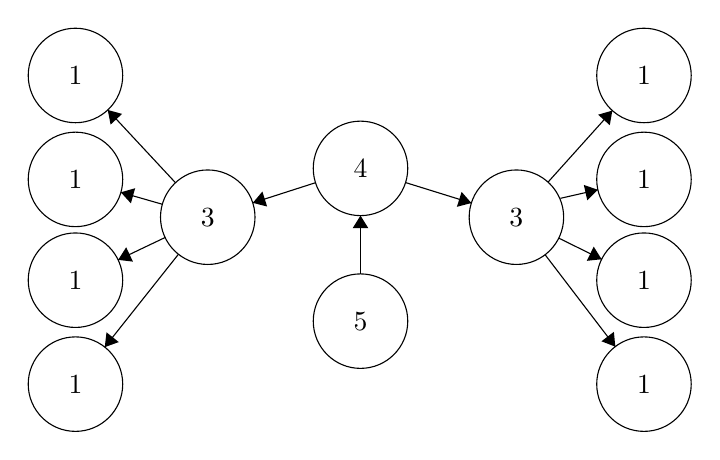
\begin{tikzpicture}[scale=0.2]
        \tikzstyle{every node}+=[inner sep=0pt]
        \draw [black] (16.1,-24.3) circle (3);
        \draw (16.1,-24.3) node {$3$};
        \draw [black] (7.7,-28.3) circle (3);
        \draw (7.7,-28.3) node {$1$};
        \draw [black] (7.7,-21.9) circle (3);
        \draw (7.7,-21.9) node {$1$};
        \draw [black] (7.7,-15.3) circle (3);
        \draw (7.7,-15.3) node {$1$};
        \draw [black] (7.7,-34.9) circle (3);
        \draw (7.7,-34.9) node {$1$};
        \draw [black] (25.8,-21.2) circle (3);
        \draw (25.8,-21.2) node {$4$};
        \draw [black] (25.8,-30.9) circle (3);
        \draw (25.8,-30.9) node {$5$};
        \draw [black] (35.7,-24.3) circle (3);
        \draw (35.7,-24.3) node {$3$};
        \draw [black] (43.8,-15.3) circle (3);
        \draw (43.8,-15.3) node {$1$};
        \draw [black] (43.8,-28.3) circle (3);
        \draw (43.8,-28.3) node {$1$};
        \draw [black] (43.8,-21.9) circle (3);
        \draw (43.8,-21.9) node {$1$};
        \draw [black] (43.8,-34.9) circle (3);
        \draw (43.8,-34.9) node {$1$};
        \draw [black] (25.8,-27.9) -- (25.8,-24.2);
        \fill [black] (25.8,-24.2) -- (25.3,-25) -- (26.3,-25);
        \draw [black] (22.94,-22.11) -- (18.96,-23.39);
        \fill [black] (18.96,-23.39) -- (19.87,-23.62) -- (19.57,-22.67);
        \draw [black] (28.66,-22.1) -- (32.84,-23.4);
        \fill [black] (32.84,-23.4) -- (32.22,-22.69) -- (31.92,-23.64);
        \draw [black] (38.5,-23.1) -- (40.87,-22.56);
        \fill [black] (40.87,-22.56) -- (39.98,-22.25) -- (40.2,-23.23);
        \draw [black] (37.71,-22.07) -- (41.79,-17.53);
        \fill [black] (41.79,-17.53) -- (40.89,-17.79) -- (41.63,-18.46);
        \draw [black] (38.39,-25.63) -- (41.11,-26.97);
        \fill [black] (41.11,-26.97) -- (40.61,-26.17) -- (40.17,-27.07);
        \draw [black] (37.52,-26.68) -- (41.98,-32.52);
        \fill [black] (41.98,-32.52) -- (41.89,-31.58) -- (41.1,-32.18);
        \draw [black] (14.24,-26.65) -- (9.56,-32.55);
        \fill [black] (9.56,-32.55) -- (10.45,-32.23) -- (9.67,-31.61);
        \draw [black] (13.39,-25.59) -- (10.41,-27.01);
        \fill [black] (10.41,-27.01) -- (11.35,-27.12) -- (10.92,-26.21);
        \draw [black] (13.22,-23.48) -- (10.58,-22.72);
        \fill [black] (10.58,-22.72) -- (11.22,-23.42) -- (11.49,-22.46);
        \draw [black] (14.05,-22.11) -- (9.75,-17.49);
        \fill [black] (9.75,-17.49) -- (9.93,-18.42) -- (10.66,-17.74);
        \end{tikzpicture}
    \end{center}
    A counter example would be as follows, given the graph $G$ in the image I provided,
    the algorithm would pick 5 first, then remove 4 and itself from $G$. The algorithm
    would then pick one of the 3 weight nodes, add it to the total, then remove the 1s
    connected to it. It would then do the same for the other 3 and 1s. In total the
    algorithm would return 11 with the set $\{5, 3, 3\} = 11$. But a better total would be
    12 with the set $\{4, 1, 1, 1, 1, 1, 1, 1, 1\} = 12$

    \hwline\part{}

    \vspace{-12pt}\hspace{20pt}Recall that a graph $G=(V,E)$ is a path if its nodes can 
    be written as $v_1,v_2,\dots,v_n$, with an edge between $v_i$ and $v_j$ if and only if
    $|i-j|=1$. Design a dynamic programming algorithm that takes an $n$-node path $G$ 
    with weights and returns an independent set of maximum weight. Show that your 
    algorithm is correct and that it runs in polynomial time.
    \hwline
    \pagebreak

    \solution
    \vspace{-28pt}\subsection{High Level Algorithm Explanation}
    \begin{enumerate}
        \item\vspace{-5pt}
        Create an include and exclude array, where each array's $i$th element shows the 
        potential maximum weight if we include or exclude the $i$th node from the maximal 
        independent set.
        \item\vspace{-5pt}
        Set the 1st element of include to the weight of the 1st node in $G$, set the
        1st element of exclude to 0.
        \item\vspace{-5pt}
        For each node $i$ from the 2nd node to the last node in $G$:
        \begin{enumerate}
            \item\vspace{-5pt}
            include[$i$] is calculated by adding G[$i$] to the max of the last 2 excluded
            node weights, this will give us the weight if we include the node at index 
            $i$ in $G$, checking the excluded previous adjacent node weights will give us 
            the included $i$th weight.
            \item\vspace{-5pt}
            exclude[$i$] is calculated by adding the max of the last include/exclude 
            weights. This will place the max weight in the exclude array, which will
            be used in the future exclude/include calculations, it represents the
            max weight if we exclude the current node.
        \end{enumerate}
        \item\vspace{-5pt}
        From $i=$ the number of nodes in $G$ to the first node (reverse through include /
        exclude):
        \begin{enumerate}
            \item\vspace{-5pt}
            If the include[$i$] value is $\ge$ to exclude[$i$], this indicates that the
            current node yields a higher total weight rather than excluding it, add to 
            the maximal independent set, then skip the next node to retain the 
            independent set property.
        \end{enumerate}
    \end{enumerate}
    \hwline
    \subsection{Time Complexity Justification}
    Initialize the two include and exclude arrays, this takes $O(n)$ time, where $n$ is 
    the number of nodes in $G$.

    \vspace{10pt}The algorithm iterates over each node in $G$ to calculate the maximal 
    weights from the include and exclude arrays, this will take $O(n)$ time.

    \vspace{10pt}The construction of the returned set requires us to iterate $n$ times
    to check each $i$th element of include and exclude, this will take $O(n)$ time.

    \vspace{10pt}Putting everything together we get the following:
    \begin{align*}
        T(n) &= O(n + n + n) \\
        T(n) &= \boxed{O(n)}
    \end{align*}
    This is polynomial to the size of the input graph $G$.
    \hwline
    \pagebreak

    \subsection{Correctness Justification}
    \hspace{20pt}This algorithm utilizes dynamic programming to compute two arrays: 
    include and exclude. The include array represents the max weight if we include
    or exclude the current node's weight. At each node $i$, the algorithm will
    consider two choices, including or excluding node $i$ from the returned set. \\

    \hspace{20pt}Each $i$th weight in include is calculated by considering the weight
    of node $i$ from $G$ plus the maximum of the previous two nodes that exclude
    their adjacent node weights. \\

    \hspace{20pt}Each $i$th weight in exclude is calculated by considering the maximum
    weight independent set of the previous node, whether it includes or excludes the
    previous node. All together this will give running weight sum if we include or
    exclude each node in the returned set of nodes. \\

    \hspace{20pt}The algorithm then iterates from the back of the include and exclude
    arrays. The algorithm adds a node to the returned set if include[$i$] yields a
    higher maximal weight if we include it rather than exclude it. It then makes sure
    to skip the next node in this reverse iteration, keeping our independent node 
    property.\\

    \hspace{20pt}Since the algorithm iterates over the nodes in reverse order, it ensures 
    that adjacent nodes are not included simultaneously in the maximum weight independent 
    set, satisfying the independence property. By selecting nodes greedily based on the 
    include and exclude values, the algorithm ensures that it maximizes the total weight 
    of the independent set.
    \hwline
    \pagebreak
    \vspace{-28pt}\subsection{Real Code Implementation}
    \begin{minted}{cpp}
// g++ -std=c++23 -O2 -Wall P2B.cpp -o P2B.exe
#include <algorithm>
#include <iostream>
#include <cstdint>
#include <vector>

std::vector<int32_t> ProblemTwoB(const std::vector<int32_t>& G)
{
    int32_t n = G.size();
    std::vector<int32_t> include(n, 0), exclude(n, 0);
    std::vector<int32_t> independentSet;

    // Base case: 
    include[0] = G[0];
    exclude[0] = 0;

    // Preprocess index 1:
    if (n > 1) {
        include[1] = G[1];
        exclude[1] = std::max(G[0], 0);
    }

    // Calculate total weights if we include/exclude each node:
    for (int32_t i = 2; i < n; ++i) {
        include[i] = G[i] + std::max(exclude[i-1], exclude[i-2]);
        exclude[i] = std::max(include[i-1], exclude[i-1]);
    }

    int32_t i = n - 1;
    while (i >= 0)
    {
        if (include[i] >= exclude[i]) {
            independentSet.push_back(i);
            i -= 2;
        } else { i--; }
    }
    return independentSet;
}
\end{minted}
\hwline
\pagebreak

\begin{minted}{cpp}
int main()
{
    std::vector<int32_t> G = {
        1, 3, 5, 20, 7, 190, 2000, 1800, -100, -2036, 1
    };
    if (G.empty()) { return -1; }
    std::vector<int32_t> maxIndependentSet = ProblemTwoB(G);

    // Print the index in G and the corresponding weight:
    std::cout << "Maximal independent set: ";
    int32_t count = 0;
    for (int32_t i = maxIndependentSet.size() - 1; i >= 0; --i)
    {
        std::cout << '\n' << maxIndependentSet[i] << ": " << G[maxIndependentSet[i]];
        count += G[maxIndependentSet[i]];
    }
    std::cout << "\nTotal weight: " << count << std::endl;
    return 0;
}
    \end{minted}
    \hwline
    \pagebreak

    \part{}

    \vspace{-12pt}\hspace{20pt} Generalize your algorithm from part $(b)$ to the case 
    where $G$ is an arbitrary tree (that is, $G$ is not necessarily a path). Show that 
    your algorithm is correct and that it runs in polynomial time. \\
    \solution
    \vspace{-28pt}\subsection{Tree Generalization}
    We should keep our include and exclude arrays (as $\langle$TreeNode*, List$\rangle$ 
    maps), each with $n$ elements, where $n$ is the number of nodes in tree $G$. \\
    Set the initial values of include to the root node's value, exclude to 0.
    \begin{enumerate}
        \item\vspace{-5pt}
        Traverse from the root node in a depth-first manner (To map values first).
        \item\vspace{-5pt}
        At each node $z$ compute the include and exclude values based on the
        child nodes of $z$.
        \begin{enumerate}
            \item\vspace{-5pt}
            For the include map value of $z$, we must consider including $z$
            by recursively adding each child's exclude value to the value of $z$.
            \item\vspace{-5pt}
            For the exclude map value we will max the include/exclude value of each
            child to $z$. Make sure to use a hashmap to retain the values.
            \item\vspace{-5pt}
            Return up the call chain.
        \end{enumerate}
        \item\vspace{-5pt}
        Now we must construct our independent set, starting from the root node
        if the include of the current node $i$ is $\ge$ to exclude[$i$],
        then add the node to the returned set, if include was $<$ than exclude, 
        then don't add $z$ to the independent set.
        \item\vspace{-5pt}
        Recursively check each child of $z$
    \end{enumerate}
    \hwline
    \subsection{Time Complexity Justification}
    My algorithm needs to traverse once to create the include and exclude maps, this will
    take $O(n)$ time, where $n$ is the number of nodes in tree $G$.

    \vspace{5pt}Constructing the maximal independent set requires us to check the include 
    and exclude values of every node, this will take $O(n)$ time.

    \vspace{5pt}All together our algorithm's time complexity is as follows:
    \begin{align*}
        T(n) &= O(n + n) \\
        T(n) &= \boxed{O(n)}
    \end{align*}
    This is polynomial to the size of the input tree $G$.
    \hwline
    \subsection{Correctness Justification}
    \hspace{20pt}The algorithm follows a similar approach as in the path case but applies 
    it to an arbitrary tree structure. \\

    \hspace{20pt}We consider the options for including or excluding each node $z$ in the 
    tree and selecting the optimal combination using the same logic and containers as in 
    the path case. At each layer we must check whether or not that node will yield us a 
    higher maximal weight over excluding it from the returned set.
    \hwline
    \pagebreak

    \subsection{Real Code Implementation}
    \begin{minted}{cpp}
// g++ -std=c++23 -O2 -Wall P2C.cpp -o P2C.exe
#include <unordered_map>
#include <algorithm>
#include <iostream>
#include <cstdint>
#include <vector>

struct TreeNode
{
    TreeNode(int32_t w) : weight(w) {}
    std::vector<TreeNode*> children;
    int32_t weight;
};

void setIncludeExclude(
    std::unordered_map<TreeNode*, int32_t>& include,
    std::unordered_map<TreeNode*, int32_t>& exclude,
    TreeNode* node)
{   // Base cases:
    include[node] = node->weight;
    exclude[node] = 0;
    // Dynamically create node's include/exclude values:
    for (TreeNode* child : node->children)
    {   // Get children values first:
        setIncludeExclude(include, exclude, child);  

        // include = exclude layer below it
        include[node] += exclude[child];
        // exclude = max(include[c], exclude[c]) (either or)
        exclude[node] += std::max(include[child], exclude[child]);
    }
}

void construct(
    std::unordered_map<TreeNode*, int32_t>& include,
    std::unordered_map<TreeNode*, int32_t>& exclude,
    std::vector<TreeNode*>& independentSet,
    TreeNode* node)
{
    if (include[node] >= exclude[node]) {
        independentSet.push_back(node);
    }
    for (TreeNode* child : node->children) {
        construct(include, exclude, independentSet, child);
    }
}
\end{minted}
\hwline

\begin{minted}{cpp}
std::vector<TreeNode*> ProblemTwoC(TreeNode* root)
{
    std::unordered_map<TreeNode*, int32_t> include, exclude;

    // Dynamically get the include and exclude values:
    setIncludeExclude(include, exclude, root);

    // Construct maximum weight independent set:
    std::vector<TreeNode*> independentSet;
    construct(include, exclude, independentSet, root);

    return independentSet;
}

int main()
{
    TreeNode* root  = new TreeNode(1111);
    TreeNode* node1 = new TreeNode(-10);
    TreeNode* node2 = new TreeNode(1535);
    TreeNode* node3 = new TreeNode(69);
    TreeNode* node4 = new TreeNode(420);

    root->children  = {node1, node2};
    node1->children = {node3, node4};

    std::vector<TreeNode*> result = ProblemTwoC(root);
    int32_t count = 0;
    std::cout << "Nodes in the maximum weight independent set:" << std::endl;
    for (TreeNode* node : result) {
        std::cout << node->weight << " ";
        count += node->weight;
    }
    std::cout << "\nMax weight: " << count << '\n';
    return 0;
}
    \end{minted}
    \hwline
\end{homeworkProblem}
\pagebreak

%%%%%%%%%%%%%%%%%%%%%%%%%%%%%%%%%%%%%%%%%%%%%%%%%%%%%%%%%%%%%%%%%%%%%%%%%%%%%%%%%%%%%%%%%

\begin{homeworkProblem}{: Counting paths.}
    \hspace{20pt}Let $G=(V,E)$ be a directed graph with no self-loops. Let $s,t\in V$ be 
    distinct vertices.
    \hwline\part{}

    \vspace{-12pt}\hspace{20pt}Design an algorithm that decides whether there exist 
    infinitely many paths from $s$ to $t$ in $G$. Note that a path is allowed to visit 
    the same vertex multiple times. Show that your algorithm is correct and that it runs 
    in polynomial time. \\
    \solution
    \vspace{-28pt}\subsection{High Level Algorithm Explanation}
    \begin{enumerate}
        \item\vspace{-5pt}
        I will create two sets that contain the visited vertices, and the current 
        vertices on the current path.
        \item\vspace{-5pt}
        My algorithm will employ a depth-first search traversal of $G$ starting from
        vertex $s$.
        \item\vspace{-5pt}
        If a cycle occurs, set a cycle flag to true indicating that a cycle has occured,
        continue delving deeper, make sure to visit every node at least once.
        \item\vspace{-5pt}
        If there are no more nodes to check, check if the cycle flag is set to
        true then return true if and only if $t$ is present in the visited set, else
        return false.
    \end{enumerate}
    \hwline
    \subsection{Time Complexity Justification}
    In the worst case, if $G$ is a directed acyclic graph, every vertex and edge must
    be visted at least once. \\This results in a time complexity of:
    \begin{align*}
        T(V, E) &= \boxed{O(V + E)}
    \end{align*}
    Given that $V$ is the number of vertices and $E$ is the number of edges in $G$.
    \\ The overall time complexity is polynomial in the size of the input graph $G$.
    \hwline
    \subsection{Correctness Justification}
    \hspace{20pt}My algorithm makes use of a well known vertex/edge traversal technique 
    called depth-first search, starting from vertex $s$. My algorithm maintains a set of
    visted vertices and the nodes on the current path, this is done to detect
    cycles. During the recursion if there is a vertex present in the current path, this
    indicates a cycle has occured, which will set the cycle flag to true. The problem 
    wants us to check if there are infinitely many paths from $s$ to $t$, this means a 
    cycle between $s$ and $t$ or a cycle before $s$ or a cycle after $t$. In all cases, 
    because my algorithm makes use of a DFS approach, it will visit every $s$ connected 
    node in the directed graph $G$.

    \hspace{20pt}The algorithm at each recursive step makes sure to backtrack when
    exploring paths, which helps ensure that each vertex is visted at least once during 
    the DFS traversal. My algorithm handles self loops by checking if that node has been
    visted before via the path set. My algorithm handles cycles likewise by checking
    if that node is present in the path set, indicating that our path looped
    back into itself, indicating a cycle, which indicates infinite paths, if our
    visited set ever contains vertex $t$.

    \hspace{20pt}Just because there is a cycle in the graph doesn't mean there is infinite
    paths from $s$ to $t$, there needs to be at least one valid path from $s$ to $t$. My
    algorithm makes use of a cycle flag while traversing and delves into new nodes, this
    is what allows my algorithm to visit every node, helping us find a single valid path
    to $t$. If the cycle flag was set to true, and $t$ is in the visited set, this means
    we have infinite paths. My algorithm will terminate due to the visited and path set
    checking if we've seen the vertex and if it's on the current path respectively.
    \pagebreak
    \vspace{-28pt}\subsection{Real Code Implementation}
    \begin{minted}{cpp}
// g++ -std=c++23 -O2 -Wall P3A.cpp -o P3A.exe
#include <iostream>
#include <unordered_map>
#include <unordered_set>
#include <vector>

bool ProblemThreeA(
    std::unordered_map<char, std::vector<char>>& G,
    std::unordered_set<char>& visited,
    std::unordered_set<char>& path,
    const char s,
    const char t)
{   // Insert new vertex into containers:
    visited.insert(s);  
    path.insert(s);
    bool cycleFound = false;

    // Check if vertex s is in G:
    if (G.find(s) != G.end())
    {   // Retrieve vertex s's neighbors:
        for (const char& neighbor : G[s])
        {
            if (path.find(neighbor) != path.end()    ||    // Cycle detected.
            (visited.find(neighbor) == visited.end() &&    // Not visted, so...
            ProblemThreeA(G, visited, path, neighbor, t))) // Delve deeper.
            {
                cycleFound = true;
            }
        }
    }
    // Backtrack current path and check if there was a cycle AND t has been found:
    path.erase(s);
    return (cycleFound && visited.find(t) != visited.end());
}

int main()
{
    std::unordered_map<char, std::vector<char>> G = {
        {'s', {'a'}},
        {'a', {'y', 'b'}},
        {'b', {'x', 's'}},
        {'t', {'z'}}  // Cycle, but no path to t: False.
    };
    std::unordered_set<char> visited, path;
    const char s = 's', t = 't';
    std::cout << ProblemThreeA(G, visited, path, s, t) << '\n';
    return 0;
}
    \end{minted}

    \pagebreak
    \part{}

    \vspace{-12pt}\hspace{20pt}Design an algorithm that computes the number of paths from 
    $s$ to $t$ in $G$, assuming there are only finitely many such paths. Note that your 
    algorithm does not have to output the paths. Show that your algorithm is correct and 
    that it runs in polynomial time.

    \solution
    \vspace{-28pt}\subsection{High Level Algorithm Explanation}
    \begin{enumerate}
        \item\vspace{-5pt}
        Create a hashtable called DP, it will have each vertice's number of paths
        from there to $t$.
        \item\vspace{-5pt}
        Set DP[$t$] to 1, the value to be returned to each node connected to
        $t$.
        \item\vspace{-5pt}
        Iterate over every vertex $v$ in $G$.
        \begin{enumerate}
            \item\vspace{-5pt}
            If $v\ne t$, set DP[$v$]$=0$, initialization for $v$ in DP.
            \item\vspace{-5pt}
            Iterate over each neighboring vertex $w$ from $v$:
            \begin{enumerate}
                \item\vspace{-5pt}
                Update the current DP value for $v$ by adding DP[$w$]'s value to DP[$v$].
            \end{enumerate}
        \end{enumerate}
        \item\vspace{-5pt}
        Return DP[$s$].
    \end{enumerate}
    \hwline
    \subsection{Time Complexity Justification}
    Because we are iterating over ever vertex and its edges, the time complexity is as 
    follows:
    \begin{align*}
        T(V, E) &= \boxed{O(V + E)}
    \end{align*}
    Given that $V$ is the number of vertices and $E$ is the number of edges in $G$.
    \\ The overall time complexity is polynomial in the size of the input graph $G$.
    \hwline
    \subsection{Correctness Justification}
    \hspace{20pt}The algorithm correctly computes the number of paths from s to t in the 
    graph by iteratively updating the DP values. By setting $t$ to 1 initally, the nodes
    neighboring $t$ will gain 1, then its neighbors will gain the value it has, multiple
    paths will have intersecting DP values to add, causing the DP value to go up by one
    for each intersecting neighbor. Returning the value of DP[$s$] at the end will
    return the number of paths, that had intersecting nodes on its path towards
    $t$. Therefore, the algorithm produces the correct result and runs efficiently,
    providing an effective solution to the problem. The algorithm will also terminate
    because the input graph $G$ must be finite.
    \hwline
    \pagebreak
    \vspace{-28pt}\subsection{Real Code Implementation}
    \begin{minted}{cpp}
// g++ -std=c++23 -O2 -Wall P3B.cpp -o P3B.exe
#include <unordered_map>
#include <unordered_set>
#include <iostream>
#include <cstdint>
#include <vector>

uint32_t ProblemThreeB(
    std::unordered_map<char, std::vector<char>>& G,
    const char s,
    const char t)
{
    std::unordered_map<char, uint32_t> DP;
    // Base case - t, increment scale factor:
    DP[t] = 1;

    // Iterate over vertices in topological order:
    for (const auto& [v, neighbor] : G)
    {   // Initialization:
        if (v != t) { DP[v] = 0; }
        for (const char& w : neighbor)
        {   // Update dp[v] by adding paths from w to t
            DP[v] += DP[w]; 
        }
    }
    // Return the number of paths from s to t
    return DP[s];
}

int main()
{
    std::unordered_map<char, std::vector<char>> G = {
        {'s', {'a', 'b'}},
        {'a', {'t'}},
        {'b', {'t'}},
        {'t', {}}
    };
    std::cout << "Number of paths from s to t: " << ProblemThreeB(G, 's', 't') << '\n';
    return 0;
}
    \end{minted}
    \hwline
\end{homeworkProblem}

%%%%%%%%%%%%%%%%%%%%%%%%%%%%%%%%%%%%%%%%%%%%%%%%%%%%%%%%%%%%%%%%%%%%%%%%%%%%%%%%%%%%%%%%%

\end{document}